\documentclass[11pt,spanish,a4paper]{article}
% Versión 2.o cuat 2015 Víctor Bettachini < bettachini@df.uba.ar >

\usepackage{babel}
\addto\shorthandsspanish{\spanishdeactivate{~<>}}
\usepackage[utf8]{inputenc}
\usepackage{float}

\usepackage{units}
\usepackage[separate-uncertainty=true, multi-part-units=single, locale=FR]{siunitx}

\usepackage{amsmath}
\usepackage{amstext}
\usepackage{amssymb}

\newcommand{\pvec}[1]{\vec{#1}\mkern2mu\vphantom{#1}}

\usepackage{tikz}
% \input{DimLinesTikz}
\usetikzlibrary{decorations.pathmorphing, patterns}

\usepackage{graphicx}
\graphicspath{{./graphs/}}
\usepackage{wrapfig}

\usepackage[margin=1.3cm,nohead]{geometry}
% \voffset-3.5cm
% \hoffset-3cm
% \setlength{\textwidth}{17.5cm}
% \setlength{\textheight}{27cm}

\usepackage{lastpage}
\usepackage{fancyhdr}
\pagestyle{fancyplain}
\fancyhead{}
\fancyfoot{{\tiny \textcopyright Departamento de Física, FCEyN, UBA}}
\fancyfoot[C]{ {\tiny Actualizado al \today} }
\fancyfoot[RO, LE]{Pág. \thepage/\pageref{LastPage}}
\renewcommand{\headrulewidth}{0pt}
\renewcommand{\footrulewidth}{0pt}

% \def \materia {Física II para químicos}
\def \periodo {cuatrimestre de verano - 2017}
\def \website {http://materias.df.uba.ar/f2qa2017v}


\begin{document}
\noindent
\textbf{Física II (Químicos)}\hfill \textcopyright {\tt DF, FCEyN, UBA}
% \textbf{\materia}\hfill \periodo
\begin{center}
  \textsc{\large Circuitos de corriente alterna - Resonancia - Potencia}
  % \textsc{\large Guía 6: Circuitos de corriente alterna - Circuito RLC - Resonancia - Potencia}
\par\end{center}{\large \par}


\begin{enumerate}
% \section*{Circuitos de corriente alterna}
% \section*{Circuito RLC}
% \section*{Resonancia - Potencia}

	% serie
	\item Una inductancia \(L\) con resistencia interna \(r\) está conectada en serie con una resistencia \(R= \SI{200}{\ohm}\).
		Cuando estos elementos están conectados a una fuente de \SI{220}{\volt} a \SI{50}{\hertz}, la caída de tensión sobre \(R\) es de \SI{50}{\volt}.
		Esta sería de \SI{44}{\volt} si la frecuencia de la fuente sería de \SI{60}{\hertz}.
	Determinar \(L\) y \(r\).


	% paralelo
	\item Un capacitor \(C= \SI{1}{\micro\farad}\) está conectado en paralelo con una inductancia \(L= \SI{0.1}{\henry}\) con resistencia interna de \SI{1}{\ohm}.
		Se conecta la combinación a una fuente alterna de \SI{220}{\volt} a \SI{50}{\hertz}.
		Determine:
		\begin{enumerate}
			\item la corriente por el capacitor,
			\item la corriente por la inductancia,
			\item la corriente total a través de la fuente,
			\item y la potencia total disipada.
		\end{enumerate}
		Construir el diagrama vectorial en el plano complejo para cada paso.


%	% no numérico, resonancia, serie
%	\item Una resistencia \(R\), un condensador \(C\) y una inductancia \(L\) están conectados en serie.
%		\begin{enumerate}
%			\item Calcular la impedancia compleja de la combinación y su valor en resonancia (esto es, cuando la reactancia \(X\) se anula).
%			\item Hallar el valor de la impedancia cuando \(|X|= \sqrt{3} R\).
%				Notar que existen dos frecuencias (\(\omega_2\) y \(\omega_1\)) para los cuales esto se cumple.
%			\item Graficar la potencia disipasada por \(R\). Cuidar de trazar la curva de resonancia y hallar el ancho de banda (\(\omega_2\ - \omega_1\)).
%			% \item Repetir los puntos anteriores suponiendo ahora que los mismos componentes se conectan en paralelo.
%		\end{enumerate}


	% admitancia
	\item Tres impedancias \(Z_1= \SI{10}{\ohm}\) , \(Z_2= \SI{20+20i}{\ohm}\) , y \(Z_3= \SI{3-4i}{\ohm} \) están conectadas en paralelo a una fuente de \SI{40}{\volt} a \SI{50}{\hertz}.
	\begin{enumerate}
		\item Calcular la admitancia, conductancia y susceptancia en cada rama,
		\item la conductancia y la susceptancia resultante de la combinación,
		\item la corriente en cada rama, la corriente resultante y la potencia total disipada,
		\item y trazar el diagrama vectorial del circuito.
	\end{enumerate}


	% circuito
	\item \begin{minipage}[t]{0.65\textwidth}
		En el circuito de la figura, la fuente de tensión \(E\) entrega \SI{100}{\volt} con una frecuencia de \SI{50}{\hertz} y los elementos que lo constituyen son: \(C= \SI{20}{\micro\farad}\), \(L= \SI{0.25}{\henry},\) y \(R_1= R_2= R_3= \SI{10}{\ohm}\).
		\begin{enumerate}
			\item Calcular la impedancia equivalente entre A y B,
			\item la corriente que circula por cada resistencia, 
			\item y construir el diagrama vectorial del circuito.
		\end{enumerate}
	\end{minipage}
	\begin{minipage}[c][1em][t]{0.3\textwidth}
		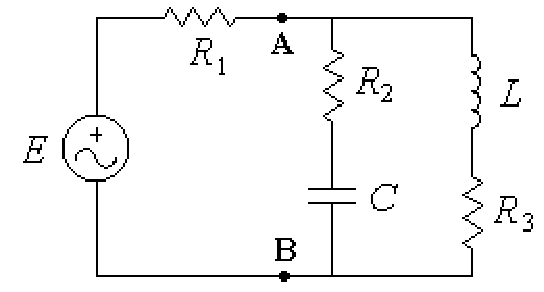
\includegraphics[width=\textwidth]{p6e05}
	\end{minipage}


	\item \begin{minipage}[t]{0.65\textwidth}
		Se reacomodaron los elementos del circuito del problema anterior. 
		\begin{enumerate}
			\item Hallar el valor de la impedancia compleja equivalente, 
			\item y determinar su valor en resonancia.
			\item ¿Cuánto es \(\omega\) en ese caso?
			\item Construir el diagrama vectorial general y de cada rama.
		\end{enumerate}
	\end{minipage}
	\begin{minipage}[c][1em][t]{0.3\textwidth}
		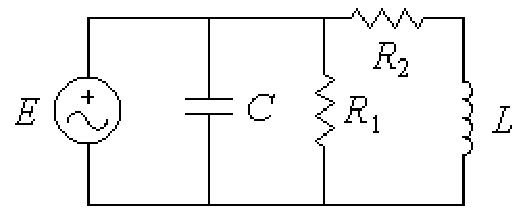
\includegraphics[width=\textwidth]{p6e06}
	\end{minipage}


	\item \begin{minipage}[t]{0.6\textwidth}
		Use el método de mallas para hallar:
		\begin{enumerate}
			\item las corrientes que circulan por cada rama,
			\item la potencia suministrada por cada generador,
			\item y la potencia disipada en cada impedancia.
		\end{enumerate}
		Datos: \(V_1= \SI{30}{\volt}\), \(V_2= \SI{20}{\volt}\), \(Z_1= \SI{5}{\ohm}\), \(Z_2= \SI{4}{\ohm}\), \(Z_3= \SI{2+3i}{\ohm}\), \(Z_4= \SI{5i}{\ohm}\), \(Z_5= \SI{6}{\ohm}\) y \(f= \SI{50}{\hertz}\).
	\end{minipage}
	\begin{minipage}[c][1em][t]{0.35\textwidth}
		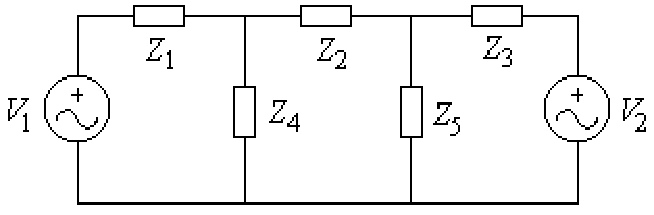
\includegraphics[width=\textwidth]{p6e07}
	\end{minipage}

	\item
    \parbox[t]{\dimexpr\textwidth-\leftmargin}{%
      \vspace{-2.5mm}
      \begin{wrapfigure}{r}{0.4\textwidth}
        \centering
        \vspace{-\baselineskip}
        % resistencia en serie inductancia, capacitor solo
        \begin{tikzpicture}[scale= .9]
            \draw (-3.5,2) -- (3,2);
            \draw (-3.5,-2) -- (3,-2);
            \draw (-3.5,2) -- (-3.5,1.5);
            \draw (-3.5,-1.5) -- (-3.5,-2);
            \draw [thick] (-3.5,1) circle (.5) node {\(A \)}; % fuente
            \draw (-3.5,-.5) -- (-3.5,.5);
            \draw [thick] (-3.5,-1) circle (.5) node {\(\sim \)}; % fuente
            \draw (-1.5,2) -- (-1.5,.75); % superior Z_1
            \draw [thick] (-1.25,0.75) node [below=18, left=11] {\(Z_1 \)} -- ++(-.5,0) -- ++(0,-1.5) -- ++(.5,0) -- cycle; % Z_1
            \draw (-1.5,-.75) -- (-1.5,-2); % inferior Z_1
            \draw (1,2) -- (1,1.25); % superior Z_2
            \draw [thick] (1,1.25) node [below=10, left=5] {\(\SI{380}{\ohm} \)} -- ++ (-.25,-.125) -- ++(.5,-0.25) -- ++(-0.5,-.25) -- ++ (.25,-.125); % resistencia
            \draw (1,-1.25) -- (1,-2); % inferior Z_2
            \draw[decoration={aspect=0.3, segment length=3, amplitude=6, coil},decorate] (1,-0.25) node [below=12,left=4] {\(\SI{541}{\milli\henry} \)} -- ++(0,-1); % bobina 
            \draw (1,.5) -- (1,-.25); % intermedia Z_2
            \draw (3,2) -- (3,-.55); % superior Z_3
            % \draw [thick] (3.25,0.75) node [below=18, left=11] {\(Z_3 \)} -- ++(-.5,0) -- ++(0,-1.5) -- ++(.5,0) -- cycle;
            \draw [ultra thick] (2.75,-.55) node [below=5,left] {\(\SI{8}{\micro\farad} \)} -- ++ (.5,0);
            \draw [ultra thick] (2.75,-0.75) -- ++ (.5,0);
            \draw (3,-.75) -- (3,-2); % inferior Z_3
        \end{tikzpicture}
	  \end{wrapfigure}
    Tres ramas comparten la misma alimentación de red (\SI{220}{\volt} diferencia de potencial efectiva, \SI{50}{\hertz}).
    % Tres ramas comparten la misma alimentación de red (\SI{311.13}{\volt} de pico, \SI{50}{\hertz}).
    Un amperímetro indica que la corriente que toman las tres es de \SI{1}{\ampere}, y su \(\cos{\varphi}=0\).
    Calcule:
    \begin{enumerate}
        \item la impedancia de la rama del capacitor,
        \item la impedancia de la rama de la bobina y la resistencia,
        \item la impedancia \(Z_1\), y
        \item la corriente en cada rama.
    \end{enumerate}
    % z1= 500- 100.j
    % i1=((0.42307692307692313+0.08461538461538462j),
    % i2= (0.4824381634677612-0.21577702286249043j),
    % i3= (-0+0.5529203070318036j))
    }


\end{enumerate}
\end{document}
